\chapter{The Effects of Feedback on Performance, Workload, and Trust in an EMG Task}
\label{chap:emg}

Portions of this chapter were originally published in the conference proceedings for AIAA SciTech 2020 \citep{doi:10.2514/6.2020-1110}.

% \documentclass[conf]{new-aiaa}
% %\documentclass[journal]{new-aiaa} for journal papers
% \usepackage[utf8]{inputenc}

% \usepackage{graphicx}
% \usepackage{amsmath}
% \usepackage[version=4]{mhchem}
% \usepackage{siunitx}
% \usepackage{longtable,tabularx}
% \setlength\LTleft{0pt}

% \title{The Effects of Training Methodology on Performance, Workload, and Trust During Human Learning of a Computer-Based Task}

% \author{Sarah M. O'Meara\footnote{Graduate Student Researcher, Mechanical and Aerospace Engineering Department.} and John A. Karasinski\footnote{Graduate Student Researcher, Mechanical and Aerospace Engineering Department, Student Member AIAA.} and Casey L. Miller\footnote{Research Assistant, Mechanical and Aerospace Engineering Department.} and Sanjay S. Joshi\footnote{Director, Robotics, Autonomous Systems, and Controls Laboratory, Professor, Mechanical and Aerospace Engineering Department.} and Stephen K. Robinson\footnote{Principal Investigator, Human/Robotics/Vehicle Integration and Performance Lab, Professor, Mechanical and Aerospace Engineering Department, Associate Fellow AIAA.}}
% \affil{University of California, Davis, Davis, CA, 95616, USA}

% \begin{document}

% \maketitle

% \begin{abstract}
% To further close the gap between human and automation, research has explored various forms of biophysical measurements for use as feedback control, such as electromyography (EMG).
% It is critical to evaluate the effects of training methodologies on performance and the evolution of workload and trust in order to achieve a seamless human-automation system.
% We developed a surface EMG control task to observe the effects of training methodology on the development of performance, workload, and trust.
% In this study, 48 subjects learned to use a surface EMG command system to perform a Fitts's Law computer-based cursor-to-target task.
% The training phase consisted of 120 Trials and the subsequent retention phase contained 40 Trials.
% Subjects were divided into four groups: Control, Concurrent Feedback, Terminal Feedback, and Adaptive Threshold.
% The Control group trained and learned through repetition using the visual feedback of the cursor position.
% The Concurrent Feedback group received additional concurrent visual feedback during command input, whereas the Terminal Feedback group had supplementary visual feedback after command input.
% The Adaptive Threshold group did not have any additional visual feedback, but experienced changes in the cursor control dynamics to induce motor learning adaptation.
% There were significant differences in percent of successfully completed trials, workload, and trust during the training phase, particularly in the earlier portion.
% The treatments were removed during the retention phase and there were no significant differences across groups.
% The results indicated that 1) there was no significant effect from the guidance hypothesis (i.e.
% the subjects did not rely on the feedback to perform the task), 2) the relationship between the subject and system evolved differently depending on the group, and 3) all training methodologies achieved similar results by the end of the study.
% We concluded that including concurrent feedback during manual task learning may provide both real-time performance improvement and an early learning plateau.
% \end{abstract}

\section{Introduction}
Biophysical monitoring during aviation operations has recently gained increased interest as a safety feature and a means to create an adaptive cockpit.
Safety-related concerns include cognitive workload~\cite{RN1, RN2}, muscle strain~\cite{RN3, RN4, RN5}, and security~\cite{RN6}.
Pilots may develop inattentional deafness to auditory alarms, but biophysical monitoring has the potential to predict these occurrences~\cite{RN7}, discriminate between cognitive loads~\cite{RN1}, and predict cognitive fatigue which results in missed auditory targets~\cite{RN2}.
The potential causes of muscle fatigue and strain has also been studied in helicopter pilots~\cite{RN3, RN4, RN5}, as well as electromyography (EMG) measurement accuracy~\cite{RN8}.
EMG has been used in aviation research to predict and warn pilots of G-Induced Loss of Consciousness~\cite{RN9, RN10}, to discriminate between novice and experienced pilots~\cite{RN11}, to control forces during emergency maneuvers~\cite{RN12}, and to command pitch and bank rates of an aircraft simulation~\cite{RN13}.
More recently, incorporating biophysical measurements has been suggested for UAV operation~\cite{RN14}.
EMG control has also been applied to robotics~\cite{RN15, RN16, RN17, RN18} with potential aerospace applications, such as tele-operations~\cite{RN19}.
In addition to tele-operations control~\cite{RN20, RN21}, EMG inputs have been used to modulate robotic arm stiffness for more precise tasks~\cite{RN22, RN23}.
While these studies have developed control strategies, they have not addressed the training aspect which is essential for the critical and complex environments found in aerospace operations.
Development of more sophisticated and integrated human-automation interfaces is clearly a trend in aviation, and more broadly in aerospace as a whole.

\subsection{Selected Training Methodologies}
Training novice users to effectively use EMG control can be a long and difficult task~\cite{RN24}.
The use of augmented feedback strategies, however, have been shown to help reduce training times.
Augmented feedback provides information that ``cannot be elaborated without an external source; thus, it is provided by a trainer or a display'' and has been shown to effectively improve performance in a wide variety of motor tasks~\cite{sigrist_augmented_2013}.
Biofeedback, which applies augmented feedback strategies to physiological signals such as EMG, has proven to be a useful tool for improving performance and assisting in rehabilitation~\cite{RN26}.
Researchers have investigated various augmented biofeedback techniques and have found them to help subjects to ``become more cognizant of their own EMG signal'', allowing for better control~\cite{RN27}.
A recent review of the biofeedback literature suggests that ``[b]iofeedback is more effective than usual therapy,'' though they also note that ``[f]urther research is required to determine the long-term effect [biofeedback has] on learning''~\cite{RN28}.

Augmented feedback can be split into two large categories describing when the feedback is presented to a subject.
Concurrent feedback is presented in real-time, as subjects complete a task, while terminal feedback is presented after the task is complete.
In general, concurrent feedback has been shown to be more useful with increasing functional task complexity, while terminal feedback is often less useful when complexity is high~\cite{sigrist_augmented_2013}.
Concurrent feedback has recently shown great promise in EMG control, though less progress has been made comparing the effects of terminal feedback strategies or investigating long-term learning effects~\cite{RN29, RN30, RN31, RN32}.

Users learn and adapt to improve performance, and surface EMG (sEMG) control adaptation may follow Bayesian theory~\cite{RN33}.
Johnson, et al.~\cite{RN33} showed significant increases in adaptation rate with increased mean error and decreased feedback uncertainty.
Noisier sEMG control methods provide richer feedback, or information about the control signal, which can lead to a larger adaptation rate compared to a more filtered classification method~\cite{RN34}.
Lyons and Joshi~\cite{RN35} demonstrated that subjects exposed to a mapping uncertainty during cursor control had larger adaptation rates when the mapping uncertainty was removed, indicating that noise during training may increase adaptation.
Inducing adaption may be a viable training methodology and has been previously shown to support generalized task learning~\cite{RN36}.

\subsection{Trust in Automation}
Trust is an important factor when considering human-automation interaction, and inappropriate trust can lead to the disuse or misuse of automated systems.
Trust is ``the attitude that an agent will help achieve an individual's goals in a situation characterized by uncertainty and vulnerability''~\cite{lee_trust_2004}.
The reliability of a system, in particular, has been shown to be an important aspect of an operator's trust in a system~\cite{RN38}.
While there have been many proposed models for trust, Hoff and Bashir's three layer model deserves particular attention~\cite{RN39}.
After performing a systematic review of the literature, they developed a three-layer model of trust which is split between dispositional trust, situational trust, and learned trust.
Though researchers have little control over dispositional trust, they can affect situational trust by varying an experimental interface or environment and learned trust can be evaluated using repeated measures.

\subsection{Recent Work}
Our recent work at University of California (U.C.), Davis includes three studies which have shown that concurrent feedback techniques can improve performance and have the potential to reduce cognitive workload in especially demanding tasks.
We investigated the effects of concurrent feedback in a simulated, four degree of freedom manually-controlled spacecraft inspection task~\cite{karasinski_real-time_2017}.
Subjects in a feedback group performed the task much faster and more accurately than those in a control group and reported a significantly lower workload.
We also investigated the effects of concurrent feedback on performance in a three-axis manual tracking task~\cite{karasinski_evaluating_2019}.
We found that subjects could use concurrent visual feedback to better learn the depth cues provided by an augmented reality headset.
Subjects were able to retain their performance improvement when the feedback was removed.
Finally, we investigated the effects of using concurrent feedback to train an aircraft flight task with variable modes of difficulty~\cite{RN42}.
Subjects exposed to the feedback immediately performed significantly better in every aspect of the task, continued this trend through the study, and retained these performance benefits after the feedback was removed in retention trials.

To the authors' knowledge, there exists no study investigating differences in performance, workload, and trust between different feedback and adaptive strategies.
In this study, we address the effects of training methodology on performance, workload, and trust during a computer-based Fitts's Law~\cite{RN43} cursor-to-target task.
The training methodologies include concurrent and terminal feedback, as well as motor learning adaptation.
Treatments are removed for the retention phase.
The goal of the study was to provide subjects with a sufficiently challenging task to observe learning effects.

\section{Materials and Methods}
\subsection{Subjects and Experimental Setup}

The U.C. Davis Institutional Review Board approved the protocol for this study, and subjects were recruited from the university student population.
Exclusion criteria for subjects included a history of neuromuscular disorders, physical limitations of dominant arm, and prior sEMG control experience.
Subjects provided written consent prior to participation.
A total of 55 subjects volunteered.
Subjects were released from the study due to equipment issues (N = 3), withdrawal request (N = 2), and significant motivation issues (e.g. not attempting the task; N = 2).
The remaining 48 subjects that completed the protocol had an average age of 20.07 years $\pm$ 1.39 years ($\mu\pm\sigma$), included 2 left-hand dominant subjects, and had equal participation of females (N = 24).

The experimental setup followed Lyons and Joshi~\cite{RN44}.
Two electrodes (ConMed 1620 Ag/AgCl center snap) approximately 2.5 cm apart were placed on the dominant hand side near the extensor digitorum proximal attachment.
A reference electrode was located near the lateral epicondyle of the humerus.
The electrodes' signal was acquired as described in Ref.~\cite{RN44}, and the signal processing followed Ref.~\cite{RN45}.
The root mean square (rms) value for each window is calculated, normalized by a manually set calibration constant, and incorporated into a moving average window (length 8) to yield an updated $\bar{x}$ at 16 Hz (used in Eq.~\ref{equation:one}).
The software for the study used the Python AxoPy library~\cite{RN46}.

\subsection{Subject Groups and Experimental Design}
Subjects proceeded through the same protocol and were assigned to one of four groups (12 subjects per group).
The four groups were each exposed to one training methodology:

\begin{enumerate}
	\item The Control group trained solely through task repetition and were able to view the motion of the cursor.
	\item The Concurrent Feedback group received additional visual feedback during the task that indicated when the processed sEMG signal exceeded a threshold value, $l_1=0.20$, which was important to selecting commands.
	\item The Terminal Feedback group received visual feedback to reflect the command that they entered.
    \item The Adaptive Threshold group was the same as the Control group with the exception that the threshold value, $l_1$, varied Trial-to-Trial between 0.10 and 0.30.
    In this group, the processed sEMG signal had to exceed a threshold that changed each trial in order to input commands.
\end{enumerate}

The protocol consisted of the following general steps: consent, entrance survey, equipment setup, experiment overview and instructions, manual calibration, Fitts's Law task and surveys for perceived workload and trust, and an exit survey.
The Fitts's Law task was divided into 16 Blocks of 10 Trials with the first 120 Trials used for training and the last 40 Trials for retention.
After each Block there was a 30 s minimum rest time during which subjects completed surveys.
In addition, a maximum voluntary contraction measurement was collected before and after the experiment to confirm that subjects were not significantly fatigued during the experiment, which has been shown to affect sEMG signals~\cite{RN47}.
We developed a ``Command Accuracy Test'' to assess each subject's ability to produce commands.
The Command Accuracy Test was conducted prior to training, at the end of training, and at the end of retention to provide an assessment similar to offline classification accuracy (see Ref.~\cite{RN48} for an EMG example).

\subsection{Fitts's Law Task}
In our study, the purpose of the Fitts's Law task was to evaluate the effects of the training methodology.
The sEMG control methodology was first presented in~\cite{RN45} and was used to command the cursor motion.
The premise of the methodology was to use serial patterns of muscle activation (``inputs'') to convey commands, similar to Morse code.
The first two inputs selected a command and the third input allowed for continuous control (See Fig.~\ref{figure:label1}a).
The command was determined based on the prior inputs with a timeout to reset in the case of errors.
In this study, subjects learned the 2-input code for four commands: up, down, left, right.
The codes were defined by the duration that the sEMG input exceeded the threshold; each input was identified as ``short'' ($\leq$ 0.50 s) or ``long'' ($>$ 0.50 s).
For example, the combination of two ``short'' inputs selected the ``up'' command.

The cursor velocity was calculated by Eq.~\ref{equation:one}, where $v_c$ was the minimum velocity (0.05 units/second), $v_m$ was the maximum velocity (0.50 units/second), $l_2$ was 0.30, and $\bar{x}$ was the filtered, averaged sEMG input.
The $l_1$ value was nominally 0.20, except for the Adaptive Threshold group in which the value was randomly selected for each Trial ($l_1 = 0.10, 0.15, 0.20, 0.25, 0.30$).

\begin{equation}
\label{equation:one}
v= v_c+\left(v_m-v_c\right)\left[\frac{\left(\bar{x}-l_2\right)}{\left(1-l_2\right)}\right]
\end{equation}

The Fitts's Law task used a center-out paradigm and similar interface as in~\cite{RN45}.
The square cursor interface had normalized horizontal and vertical bounds of [-1,1] and a length of 2 units.
Each Trial began with the cursor at the center of the interface and a target in a randomized position.
There were 40 unique target positions that covered a range of Index of Difficulties (IDs) from 1.00 to 4.09 bits (calculated by the Shannon formulation~\cite{RN50}).
The subject used sEMG to convey commands and moved the cursor to the target.
The cursor had to dwell on the target for 1 s to successfully complete the trial.
The maximum Trial time was 60 s, which was determined by reviewing data from Ref.~\cite{RN45} and preliminary testing.
As shown in Fig.~\ref{figure:label2}, the Control, Concurrent Feedback and Adaptive Threshold groups viewed similar interfaces.
The additional visual feedback in the Concurrent Feedback group was provided by changing the color of the cursor (Fig.~\ref{figure:label2}b).
The Terminal Feedback group had additional visual elements at the edges of the cursor interface that changed color to reflect the command (Fig.~\ref{figure:label2}c).
The visual feedback was displayed according to the timing shown in Fig.~\ref{figure:label1}b.

\begin{figure}[hbt!]
\centering
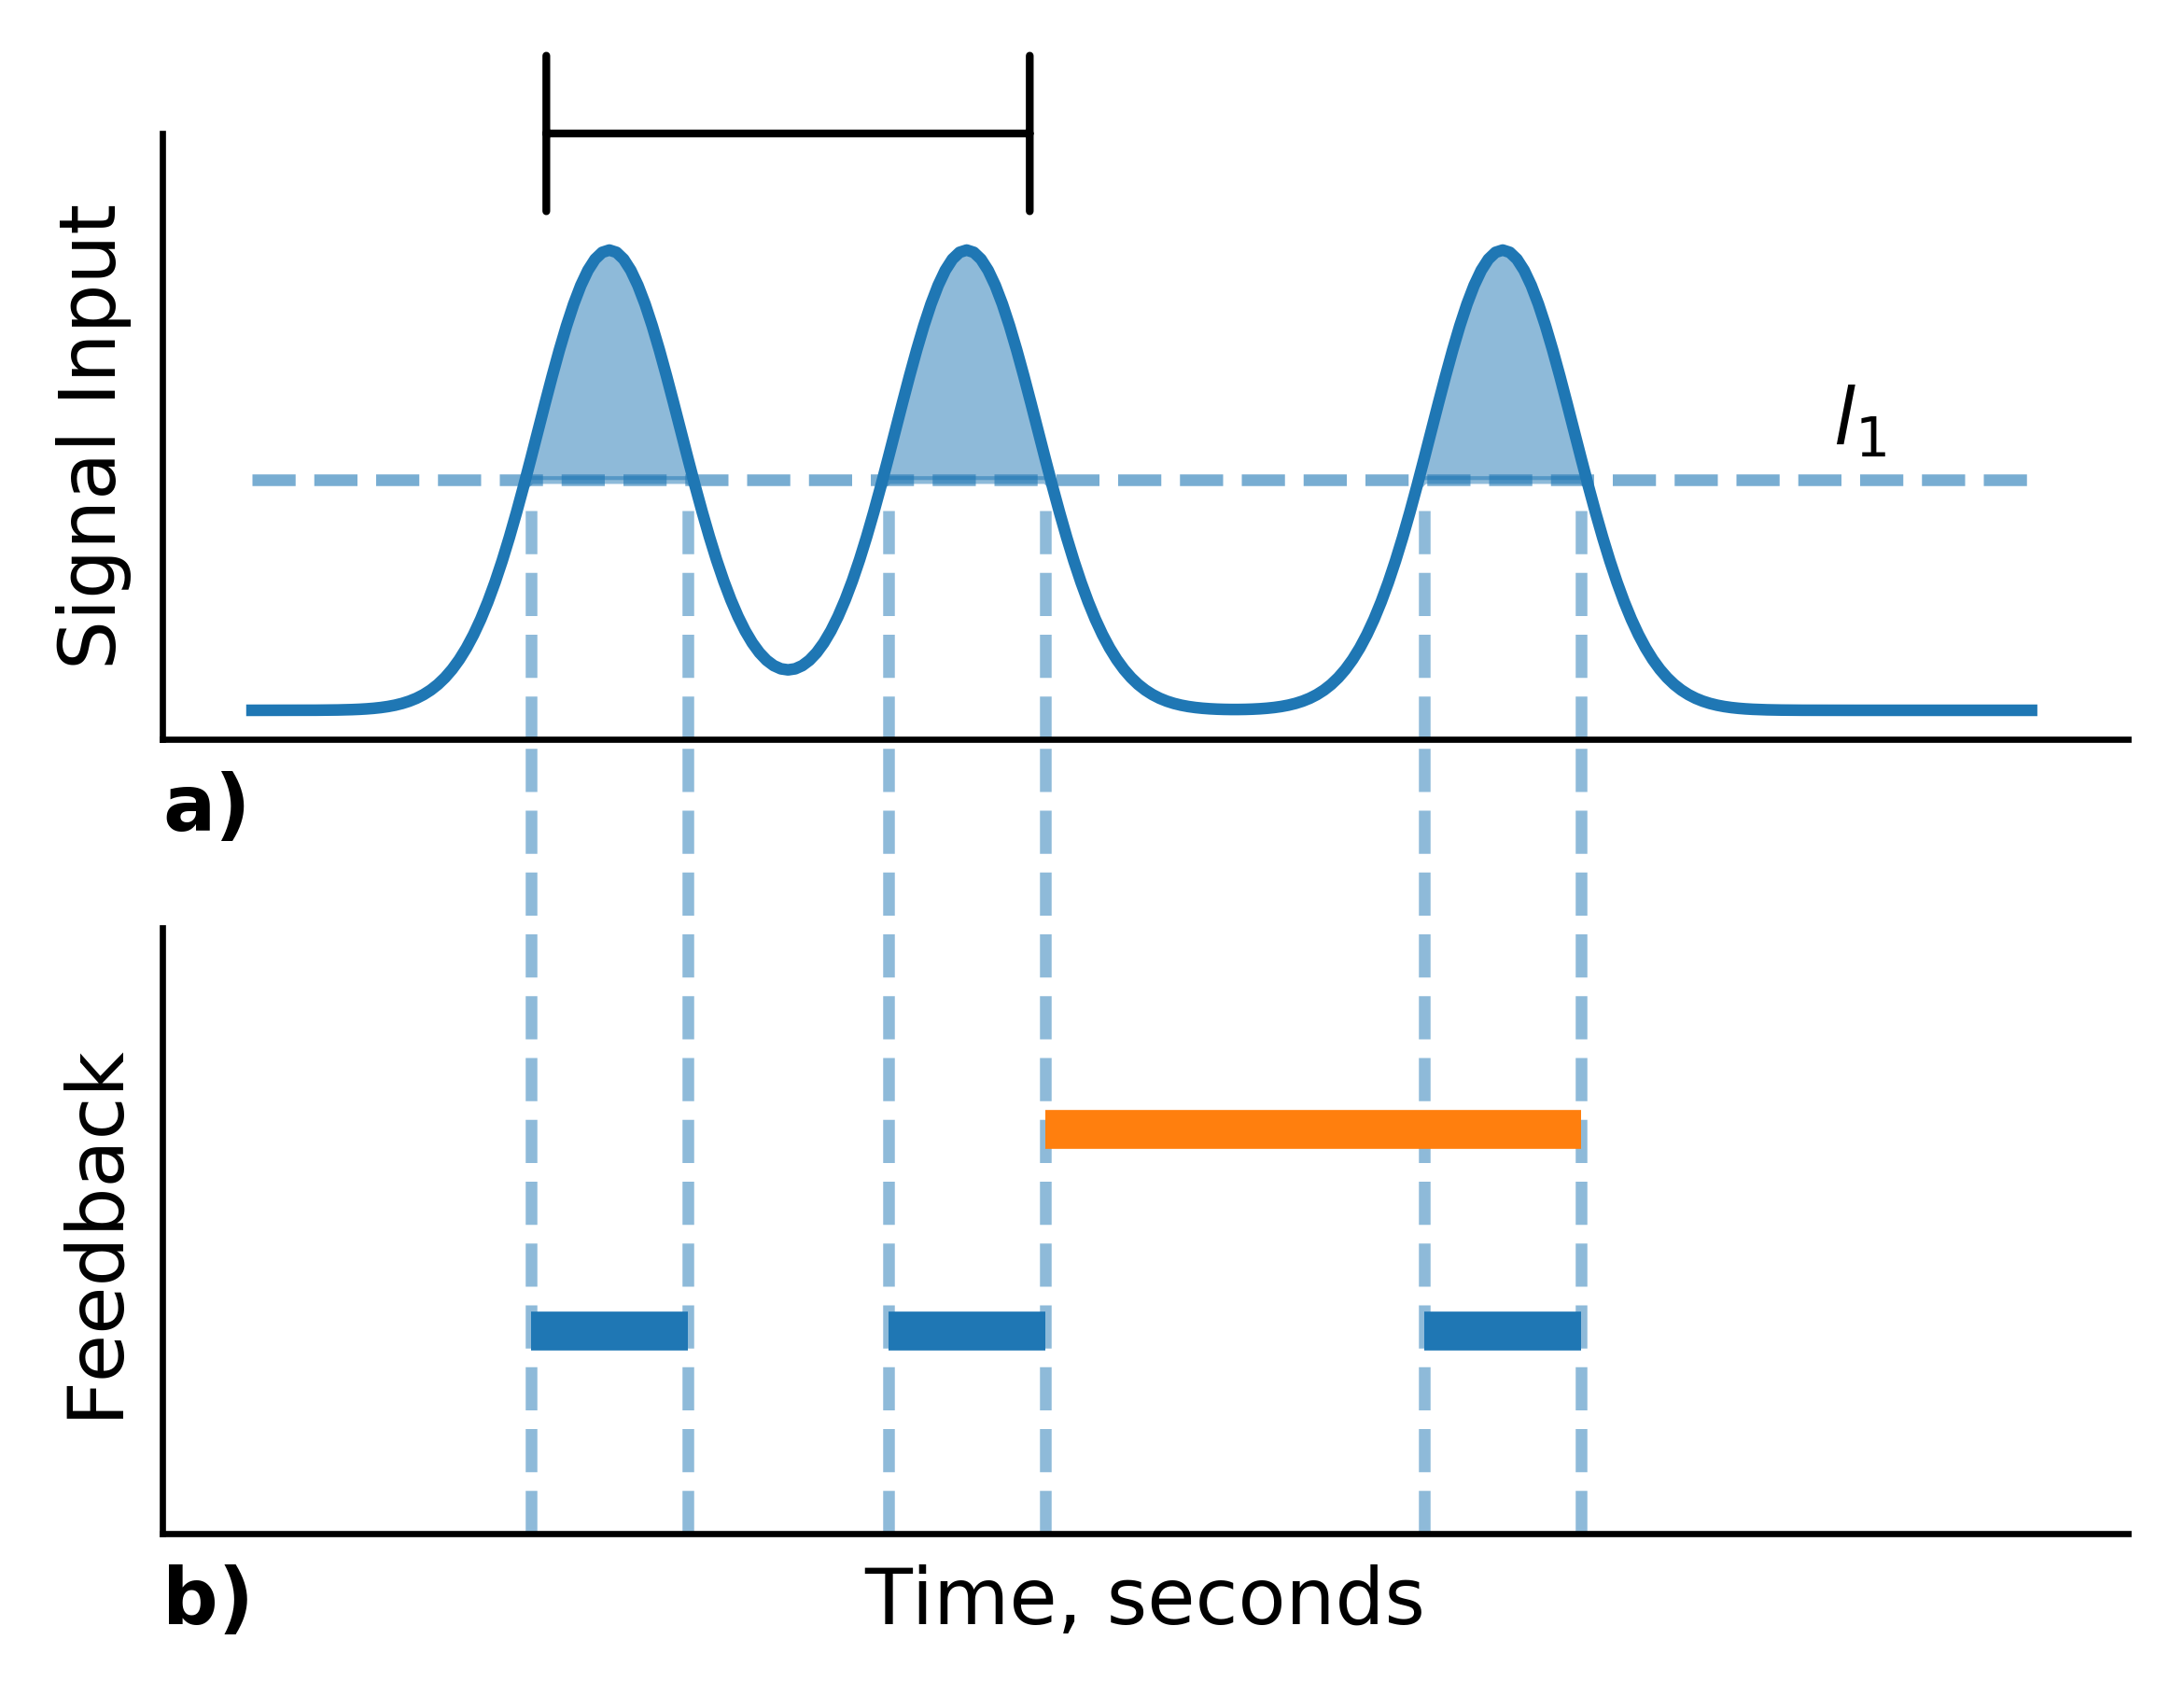
\includegraphics[height=.4\textwidth]{figures/Figure1}
\caption{\label{figure:label1} Illustrative signal input over time.
a) The first two inputs select the command; the black bar represents the command time.
The third input causes motion.
The shaded areas indicate when the signal crosses the minimum threshold, $l_1$.
b) Visual feedback is presented according to the bars (blue = Concurrent Feedback, orange = Terminal Feedback).}
\end{figure}

\begin{figure}[hbt!]
\centering
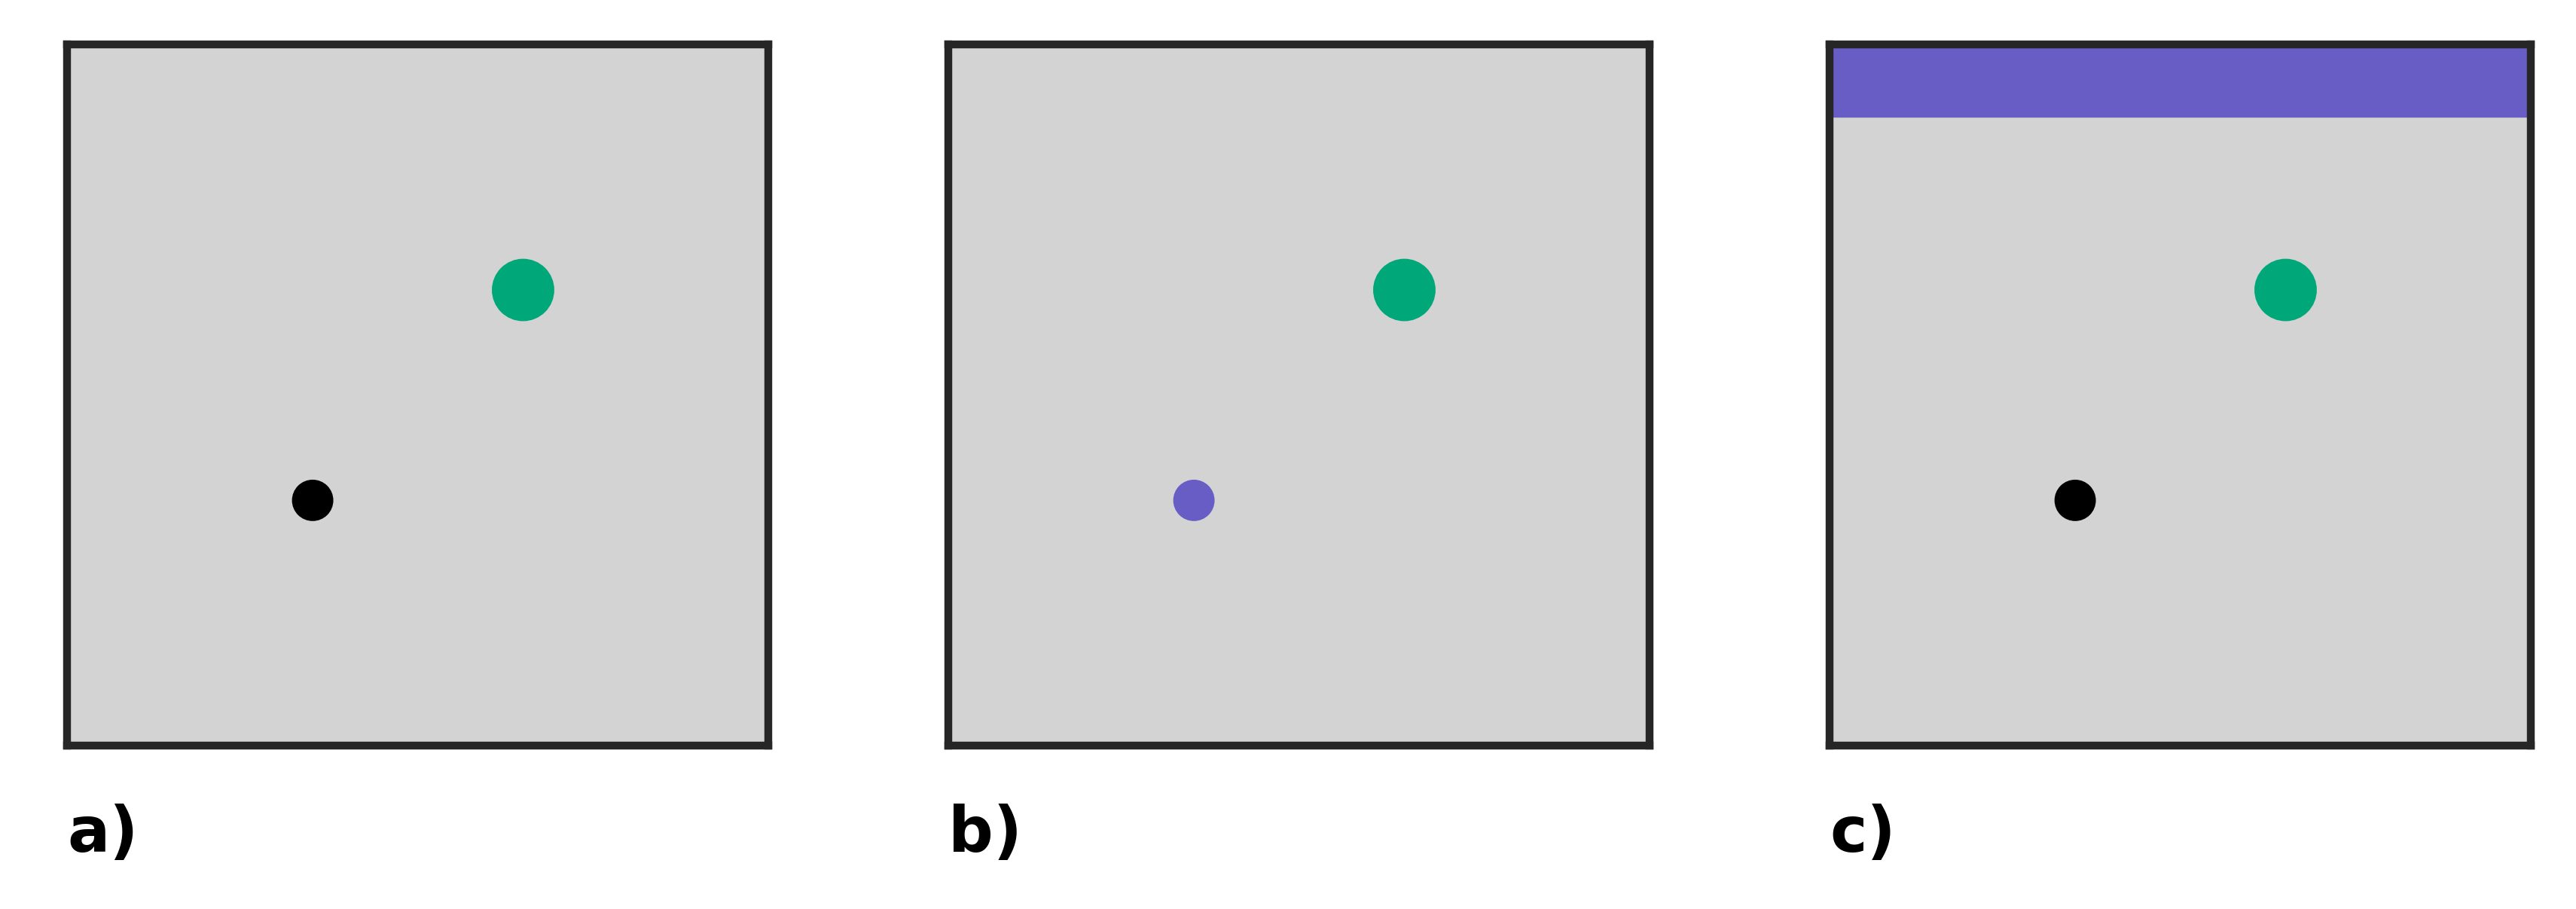
\includegraphics[width=.6125\textwidth]{figures/Figure2}
\caption{\label{figure:label2} Cursor interfaces for a) the Control and Adaptive Threshold, b) Concurrent Feedback and c) Terminal Feedback groups (not to scale).
The feedback displayed in c) indicates the ``up'' command.
Concurrent Feedback and Terminal Feedback groups see their respective displays when the feedback is activated, otherwise like a).
The target is shown in green and the cursor is the other, smaller circle.}
\end{figure}

\section{Analysis and Hypotheses}
The analysis focused on performance, workload and trust metrics to observe the effects of the training methodology.
A brief description of the analysis is provided in the following subsections.

\subsection{Performance Metrics}
The percent of successful Trials within each Block was used as the primary performance metric.
Other metrics included throughput and average trial time.
Throughput, $TP$, is a common metric from Fitts's Law defined as $TP = \frac{ID}{MT}$, where $ID$ is the Index of Difficulty and $MT$ is the Movement Time.
Average trial time was defined as the time from the start of the Trial to the Trial completion but does not include the 1 s dwell time.

\subsection{Trust and Perceived Workload}
Trust was evaluated using Jian et al.'s twelve statement questionnaire which measures trust between people and automated systems~\cite{jian_foundations_2000}.
Each of the twelve statements was evaluated on a seven-point Likert-type scale.
Perceived workload was measured using Modified Bedford scale~\cite{roscoe_subjective_1990}.
Subjects completed these surveys after each Block.

\subsection{Command Accuracy Test}
This metric quantified how accurately subjects could convey requested commands.
During the Command Accuracy Test, subjects performed each command 5 times when prompted for a total of 20 commands in a randomized order.
Each command input matching the requested command was scored as successful.
The metric was the percent of successful commands.
Subjects completed the Command Accuracy Test prior to training, after training, and after retention.

\subsection{Hypotheses}
Based on our prior experience with augmented feedback and sEMG cursor control, we formed the following hypotheses.

\begin{enumerate}
	\item During the training phase, the Concurrent Feedback group will have the highest performance followed by Terminal Feedback, then Control, and finally the Adaptive Threshold groups.
	\item All groups will perform similarly in the retention phase.
    \item The Concurrent Feedback and Terminal Feedback groups will have a high level of trust during training with some decrease during retention.
    Although, the trust level will still remain high during retention.
	\item The Control group's trust will continually increase.
	\item The Adaptive Threshold group will have lower trust during training, which will increase in retention.
	\item The perceived workload will continually decrease during the training phase for all groups with the largest decreases for the Concurrent Feedback and Terminal Feedback groups.
    \item There will be no significant difference in workload in the retention phase for all groups.
\end{enumerate}

\section{Results}
Subjects were evenly divided into four groups: Control, Concurrent Feedback (visual feedback when $\bar{x}> l_1$), Terminal Feedback (visual feedback when command selected), and Adaptive Threshold ($l_1$ varied on a Trial-by-Trial basis).
Subjects completed a total of 16 Blocks comprised of 10 cursor-to-target Trials, for a total of 160 Trials over the course of the study.
When applicable for analysis, sets of 4 Blocks were grouped into a Session.
Each Session was identical, such that the Blocks and Trials within them were identical, and the Trials randomized within the Blocks for varied target positions.
Muscle fatigue did not appear to alter the results, since the maximum voluntary contraction was not significantly different between the beginning and end of the study ($F(1, 46) = 2.55, p = 0.11$)\footnote{One subject was removed from this analysis as they changed their arm position/contraction method during testing, which affects the signal.}.

We ran two-factor mixed models to investigate changes in performance, workload, and trust with one between-subjects factor, Group, and one within-subjects repeated measure, Block.
When significant effects were observed, post hoc comparisons using the Tukey Honest Significance Difference (HSD) test were performed and considered significant at the $p < 0.05$ level, and the Satterthwaite method was used to calculate the degrees of freedom.

\subsection{Performance Metrics}
The percent success metric measured the percentage of successfully completed Trials within a Block; a Block contained 10 Trials.
There were significant main factors of Group ($F(3, 44) = 8.18, p < 0.001$) and Block ($F(15, 660) = 31.80, p < 0.001$).
There was also a significant interaction effect between Group and Block ($F(45, 660) = 3.90, p < 0.001$).
Despite the presence of an interaction effect that resulted from subjects learning the task (as indicated by the Block factor), the main effect of Group could still be interpreted.
A Tukey test showed that the subjects in the groups differed significantly, with subjects in the Concurrent Feedback group performing significantly better than those in the Control group ($p = 0.020$).
The Tukey test also showed that subjects in the Adaptive Threshold group performed significantly worse than those in the Terminal Feedback and Concurrent Feedback groups ($p < 0.001, 0.01,$ respectively).

\begin{figure}[hbt!]
\centering
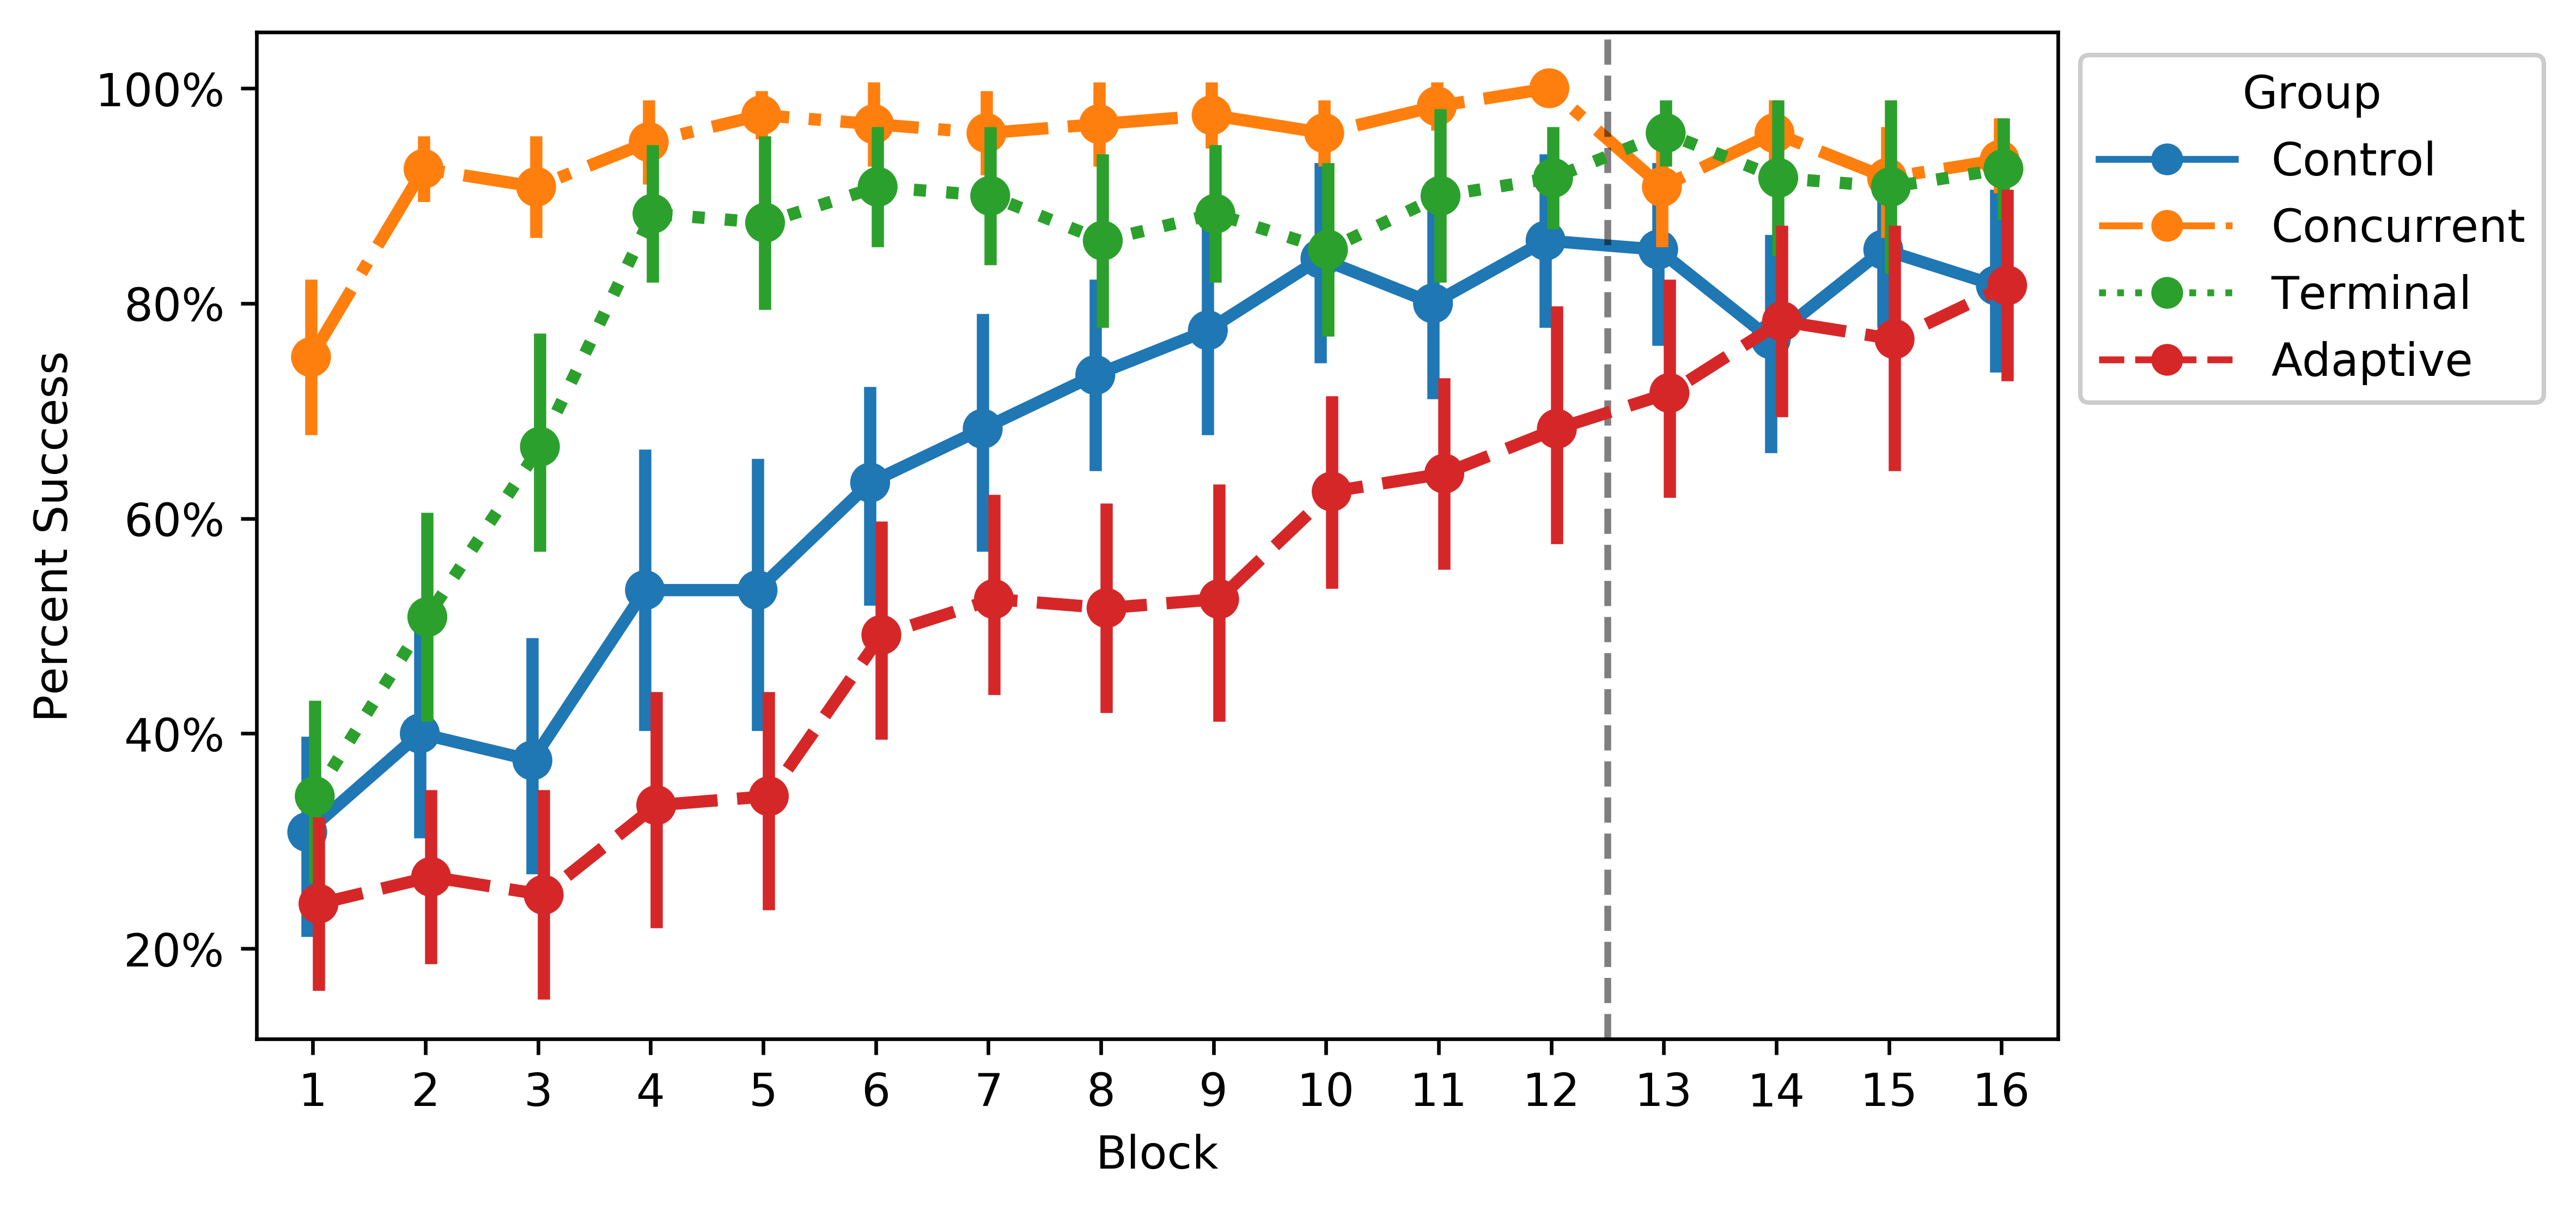
\includegraphics[height=.4\textwidth]{figures/PercentSuccess}
\caption{\label{figure:label3} Percent success by Block across groups.
The vertical dashed line represents the transition from the training phase to the retention one.
Error bars shown are the standard error of the mean.}
\end{figure}

The interaction effect resulted from different learning rates between the groups (see Fig.~\ref{figure:label3}), where subjects learned in the following order (fastest to slowest): Concurrent Feedback, Terminal, Control, and Adaptive Threshold.
Compared to the Control group, the Concurrent Feedback group significantly outperformed them for the first 6 Blocks.
Unlike the Concurrent Feedback group, the Terminal Feedback and Adaptive Threshold groups started with the same initial performance as the Control group.
The Terminal Feedback group learned more quickly than the Control group, however, and significantly outperformed the Control group for Blocks 4 and 5.
Compared to the Control group, all groups performed at statistically similar level after Block 6.
Investigating the immediate retention effects when the group-specific treatments are removed in Block 13, the mixed model showed no change in performance for any of the groups ($p > 0.99$ for all groups).
As such, the percentage of successfully completed Trials did not show any effect from the guidance hypothesis (i.e. the subjects did not rely on the feedback to complete the task and removing the feedback did not result in decreased performance).

The throughput was calculated for the retention phase and averaged across Blocks 13 through 16 (i.e. Session 4).
Throughput is generally used to asses an input device, which should be measured when the subjects can complete the task.
Since there were no significant differences in the retention phase for percent complete, it was logical to only calculate throughput at this time.
There was no significant difference in throughput between the Groups ($F(3, 44) = 1.62, p < 0.20$).
The mean throughput for all subjects was found to be 0.56 $\pm$ 0.02 bits/s ($\mu\pm\sigma$).

The randomization of the 40 target positions occurred over 4 Blocks, thus it seemed appropriate to average Trial time over a Session (i.e. set of 4 Blocks).
Trial time was only defined for successfully completed Trials, and the Satterthwaite method was used to calculate the adjusted degrees of freedom using the lmerTest package in R~\cite{RN53}.
The results are displayed in Fig.~\ref{figure:label4}.
There were significant main factors of Group ($F(3, 43.97) = 4.39, p < 0.01$) and Session ($F(3, 131.07) = 24.91, p < 0.001$).
The interaction effect between Group and Session was not significant ($F(9, 131.07) = 0.78, p = 0.63$).
A Tukey test showed that the Concurrent Feedback group performed significantly better than those in the Adaptive Threshold group ($p = 0.004$), which was the only significant difference between groups.
No groups significantly outperformed the Control group.
Analysis of the Session factor showed increased performance ($p < 0.05$) until the last two Sessions, which were not statistically different ($p = 0.65$).
These results further supported that the guidance hypothesis did not occur.

\begin{figure}[hbt!]
\centering
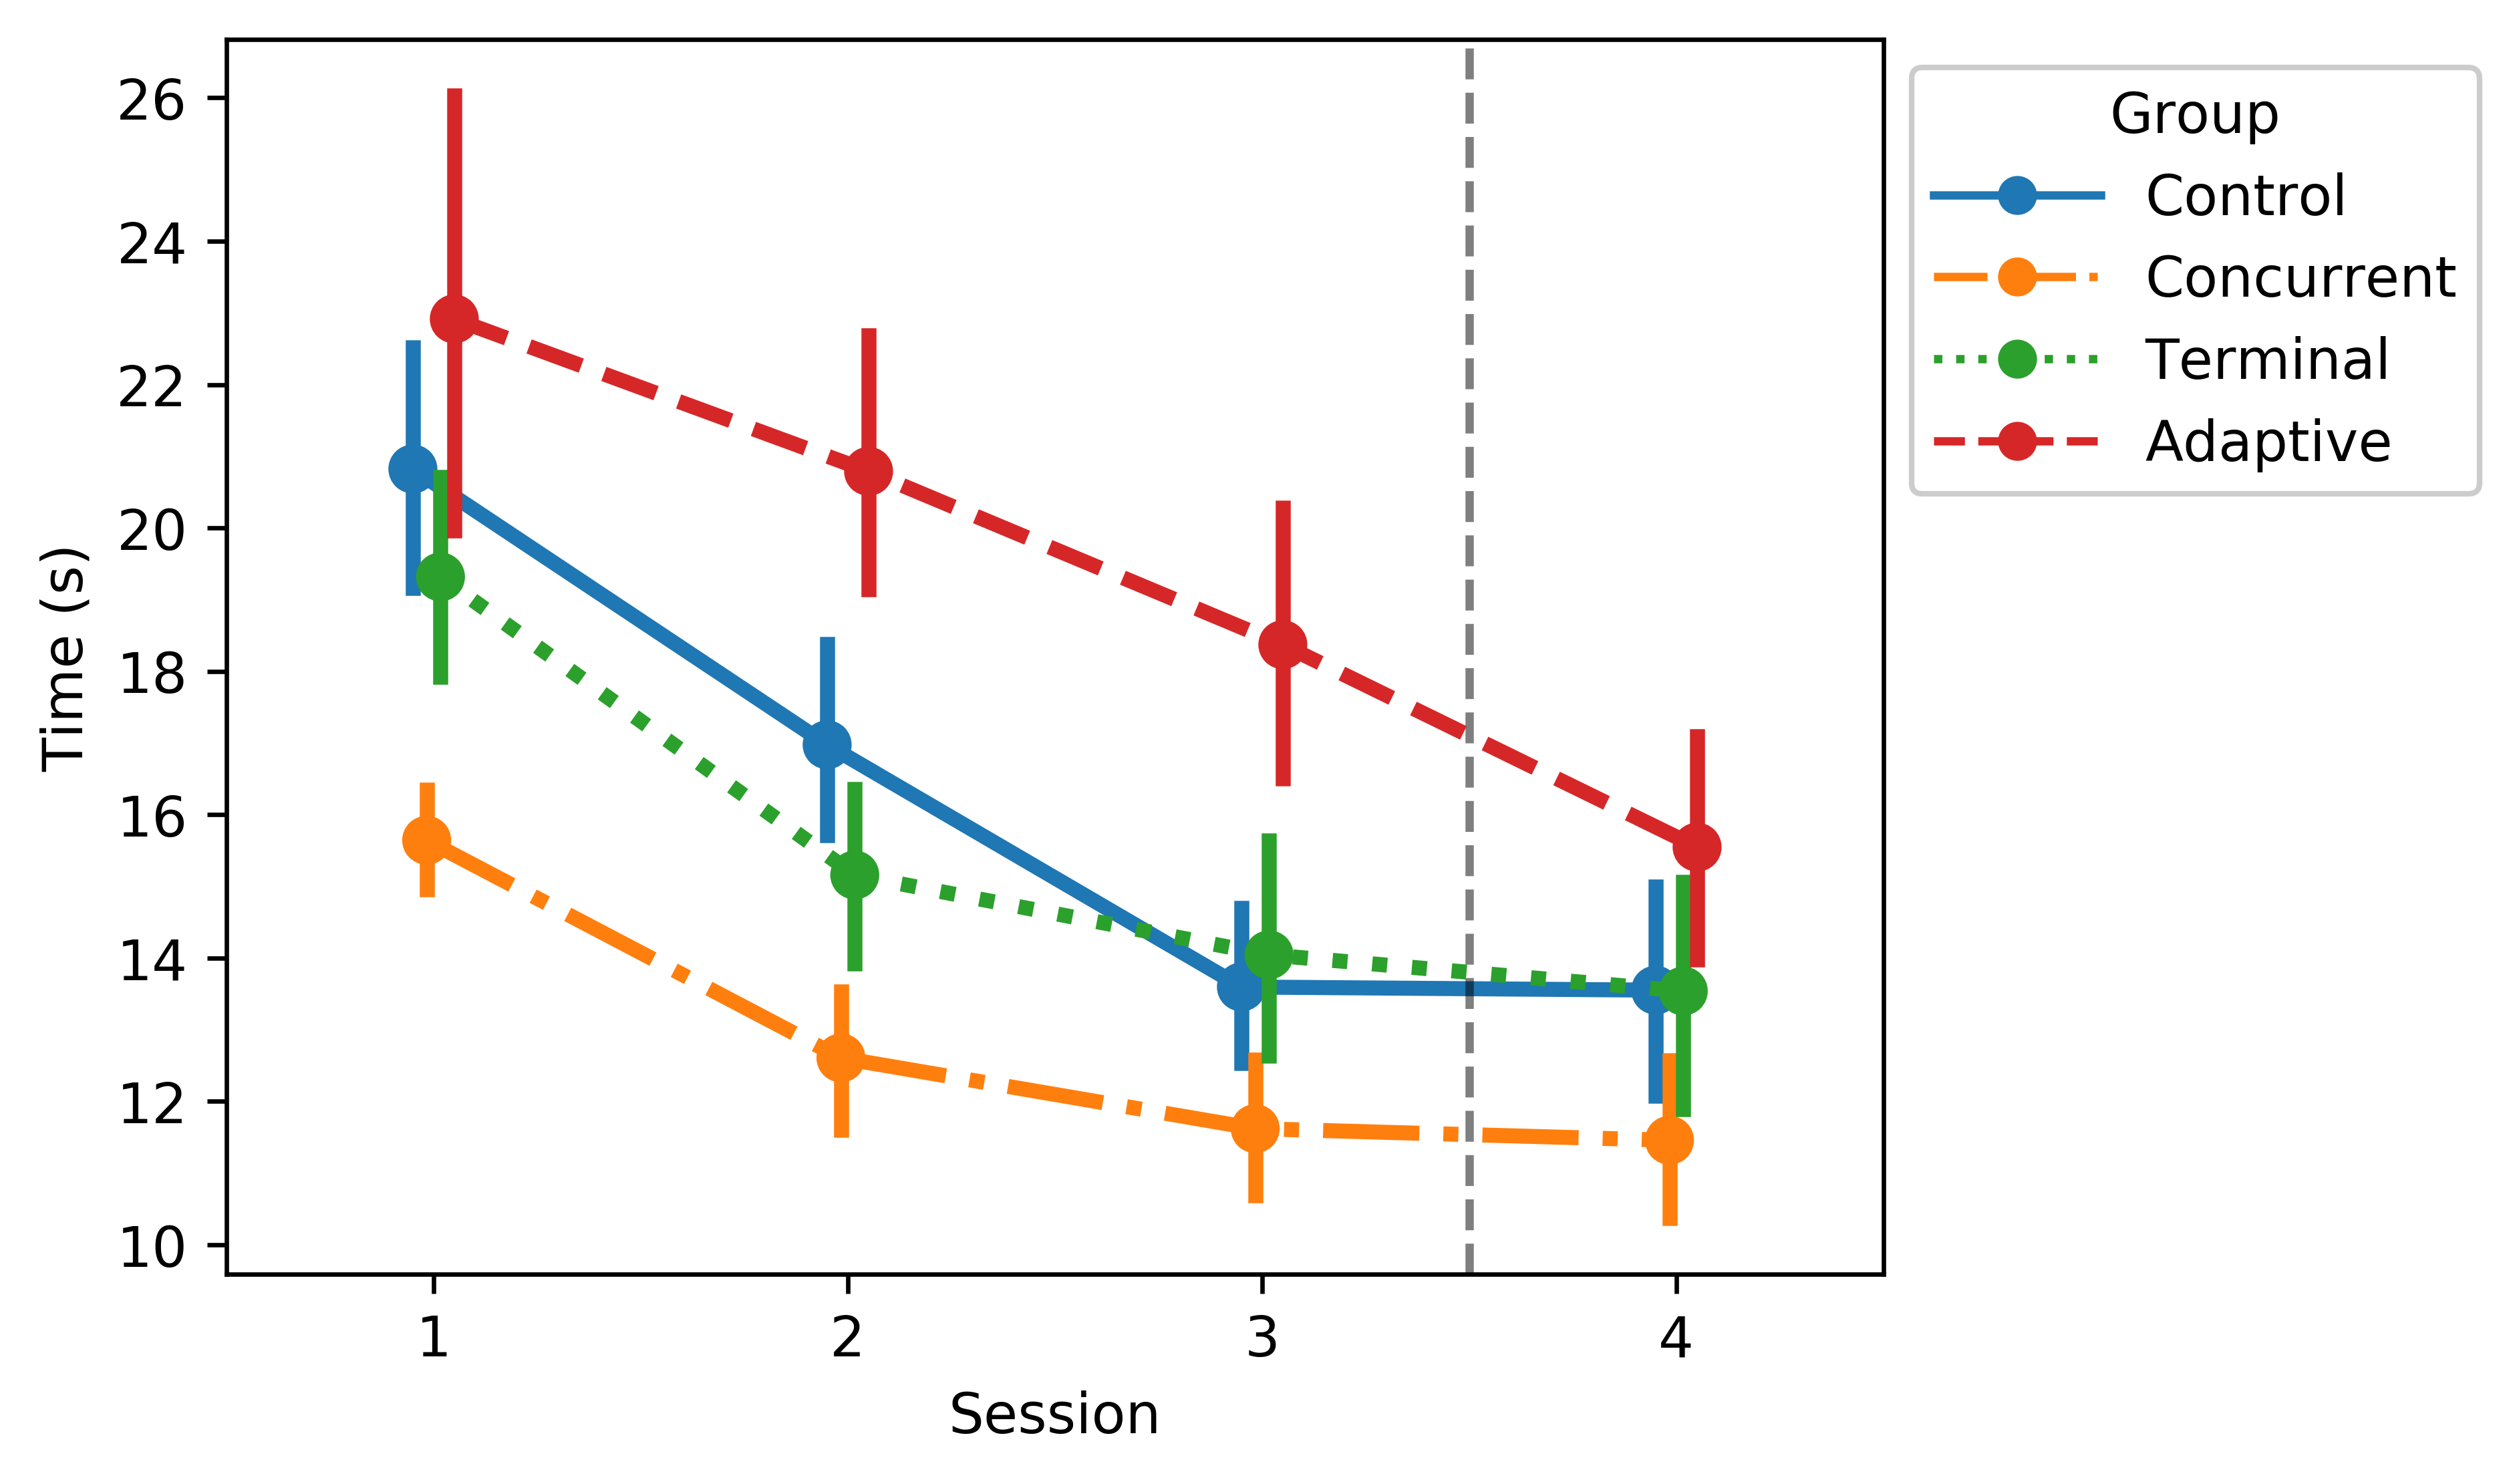
\includegraphics[height=.4\textwidth]{figures/TrialTime_session}
\caption{\label{figure:label4} Average Trial time by Session (sets of 4 Blocks) across groups.
The vertical dashed line represents the transition between the training and evaluation phases.}
\end{figure}

\subsection{Trust and Perceived Workload}
The Modified Bedford Workload metric is a subjective measurement of perceived workload that ranges from 1-10, where 1 indicates low workload and 10 indicates high workload.
There was a significant main factor of Block ($F(15, 660) = 18.29, p < 0.001$), but Group was not found to be significant ($F(3, 44) = 2.16, p = 0.106$).
There was also a significant interaction effect between Group and Block ($F(45, 660)= 1.82, p = 0.001$) (see Fig.~\ref{figure:label5}).
The interaction effect resulted from subjects reporting lower workload as they learn the task at different rates, as indicated by the Block factor.
In further investigation of the interaction, we observed that the Adaptive Threshold group reported a significantly higher workload than the Concurrent Feedback group for Blocks 9, 10, and 11.
This perception of high workload may possibly have resulted from the significantly worse performance of the Adaptive Threshold group.
None of the groups showed a significant difference in workload compared to the Control group and all four groups reported statistically similar workloads in the retention phase.

\begin{figure}[hbt!]
\centering
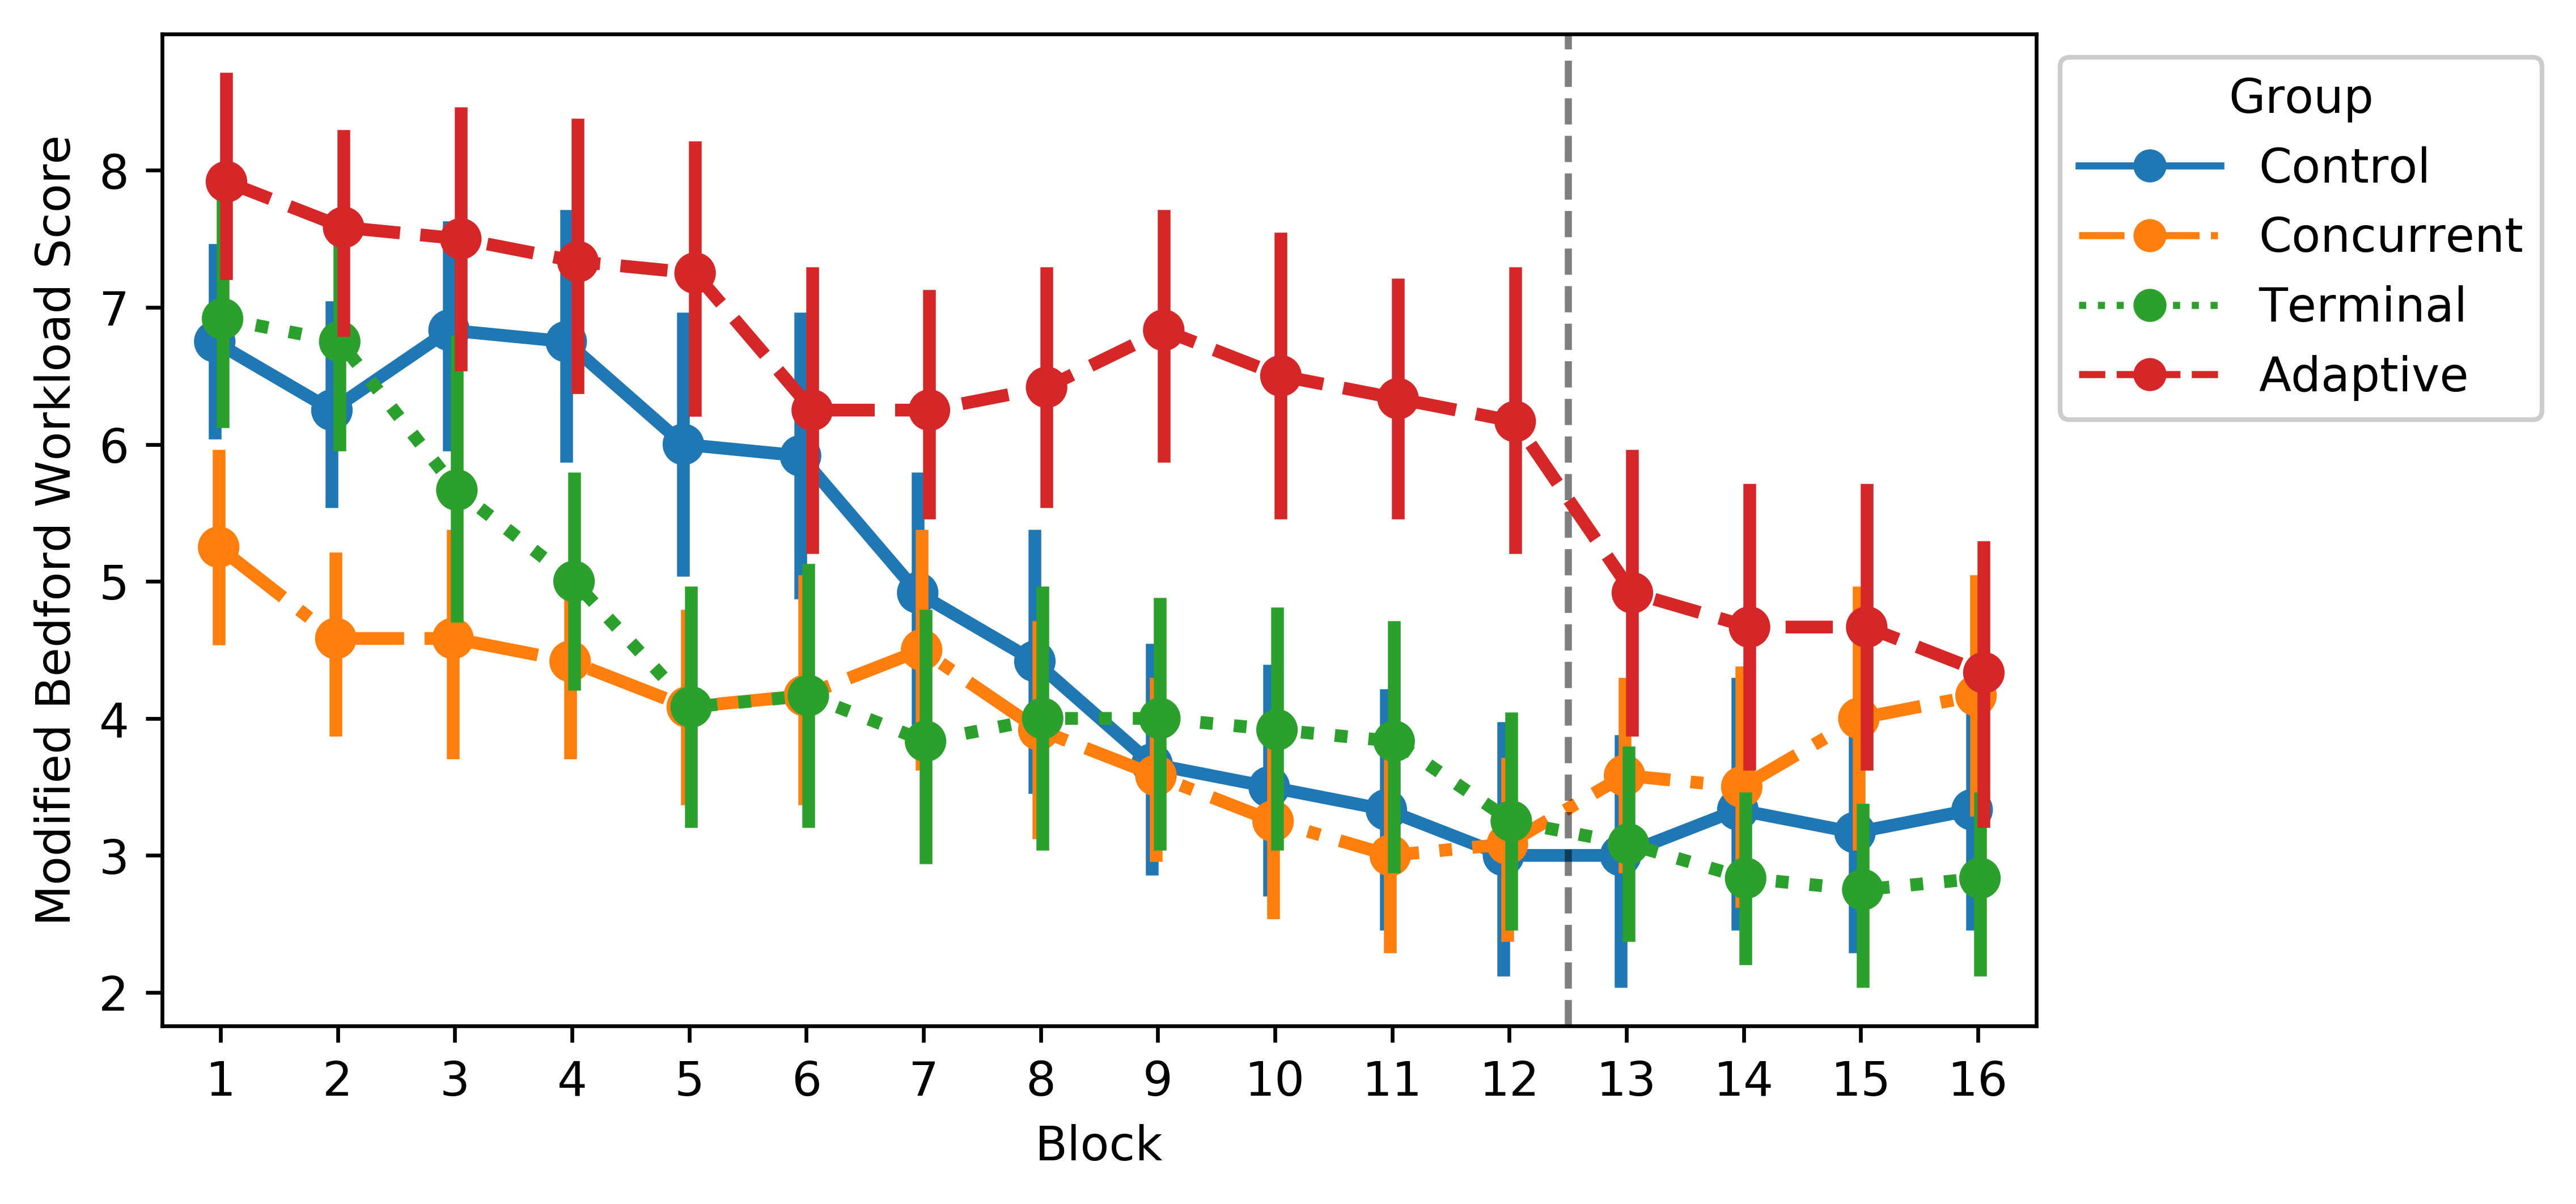
\includegraphics[height=.4\textwidth]{figures/ModifiedBedfordWorkloadScore}
\caption{\label{figure:label5} Modified Bedford Workload Score by Block across groups.
The vertical dashed line represents the transition from the training phase to the retention one.
Error bars shown are the standard error of the mean.}
\end{figure}

Intragroup changes in workload were also of interest.
The Concurrent Feedback group showed no statistically significant changes in performance between Blocks, though they did demonstrate a nonsignificant, increasing workload trend in the retention phase of the experiment.
The Terminal Feedback group had statistically higher initial workload for Blocks 1, 2, and 3, but the remainder of the Blocks had a statistically similar level of workload.
The Control group's workload was significantly higher for Blocks 1-6, possibly due to their slower learning rate, but leveled off for the remainder of the Trials.
Finally, the Adaptive Threshold group reported the highest workload in Blocks 1-5, but also saw the largest improvement transitioning into the retention phase where their $l_1$ threshold stabilized to the same fixed value as the other groups.

Trust was measured using Jian's twelve question trust survey~\cite{jian_foundations_2000}.
Each question was rated on a 7-point Likert scale, the five reverse coded questions were reversed, and the results were averaged to create a single trust score (see Fig.~\ref{figure:label6}).
There was a significant main factor of Block ($F(15, 660) = 13.05, p < 0.001$), but Group was not found to be significant ($F(3, 44) = 2.59, p = 0.065$).
There was also significant interaction effect between Group and Block ($F(45, 660) = 2.00, p < 0.001$).
The significant main effect of Block showed a gradual increase in trust throughout the duration of the study.
After investigating the interaction effect, we saw that no group reported a significantly different trust level than the control group on any Block, but that the Adaptive Threshold group recorded a significantly lower trust than the Concurrent Feedback group on Blocks 3-6 and 9.
Similar to workload, the primary interaction effects appeared driven by intragroup differences.
The Concurrent Feedback group showed no statistically significant changes through the study, the Terminal Feedback and Control groups displayed significant increases in trust in Blocks 1-6, and the Adaptive Threshold group reported significantly higher trust in the retention Session than during early Blocks.

\begin{figure}[hbt!]
\centering
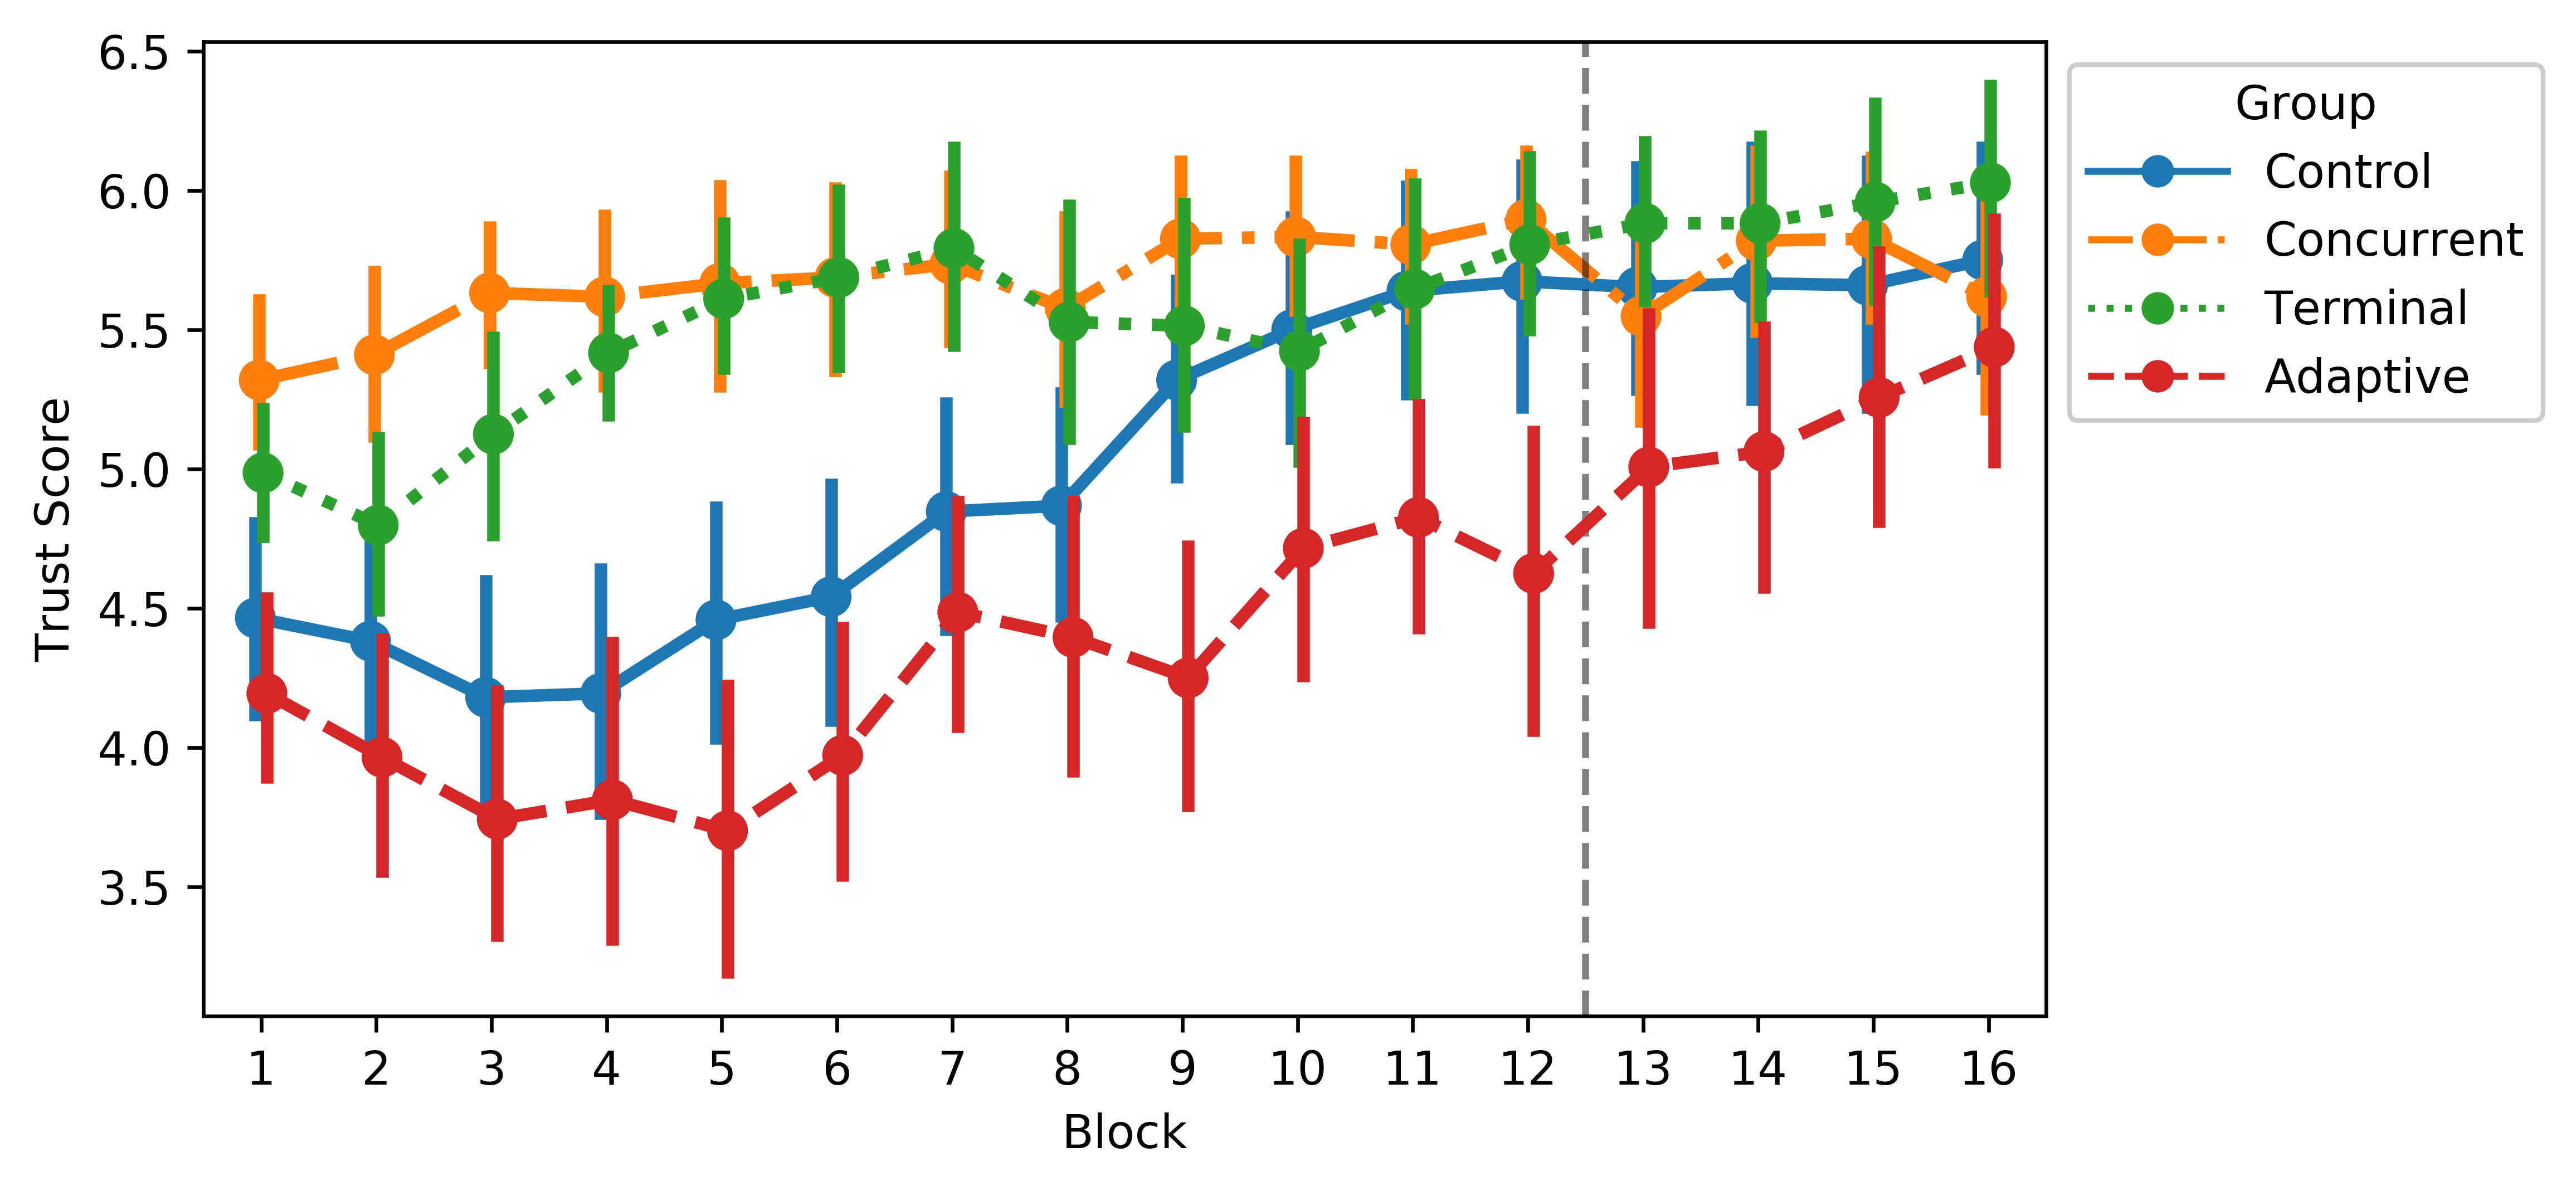
\includegraphics[height=.4\textwidth]{figures/TrustScore}
\caption{\label{figure:label6} Trust Score by Block across groups.
The vertical dashed line represents the transition from the training phase to the retention one.
Error bars shown are the standard error of the mean.}
\end{figure}

\subsection{Command Accuracy}
In contrast to previous results, the results in this section are not reported by Block or Session.
The Command Accuracy Test occurred three times (before Block 1, after Block 12, and after Block 16), and the average was calculated for each Test.

In each Command Accuracy Test, subjects responded to prompts to perform commands.
The command accuracy percent indicates the percentage of the 20 prompts in each Test that subjects correctly performed.
Results were averaged by group (see Fig.~\ref{figure:label7}).
There was a significant main factor of Test ($F(2, 88) = 108.48, p < 0.001$), but Group was not significant ($F(3, 44) = 2.63, p = 0.06$).
The interaction effect between Group and Test was not significant ($F(6, 88) = 0.82, p = 0.55$).
Investigation into the Test variable showed that subjects performed significantly better between Test 1 and 2, and between Test 1 and 3, but not between Test 2 and 3.
These results demonstrated that there was a significant improvement in the percent of commands accurately entered after the training portion of the experiment was finished.

\begin{figure}[hbt!]
\centering
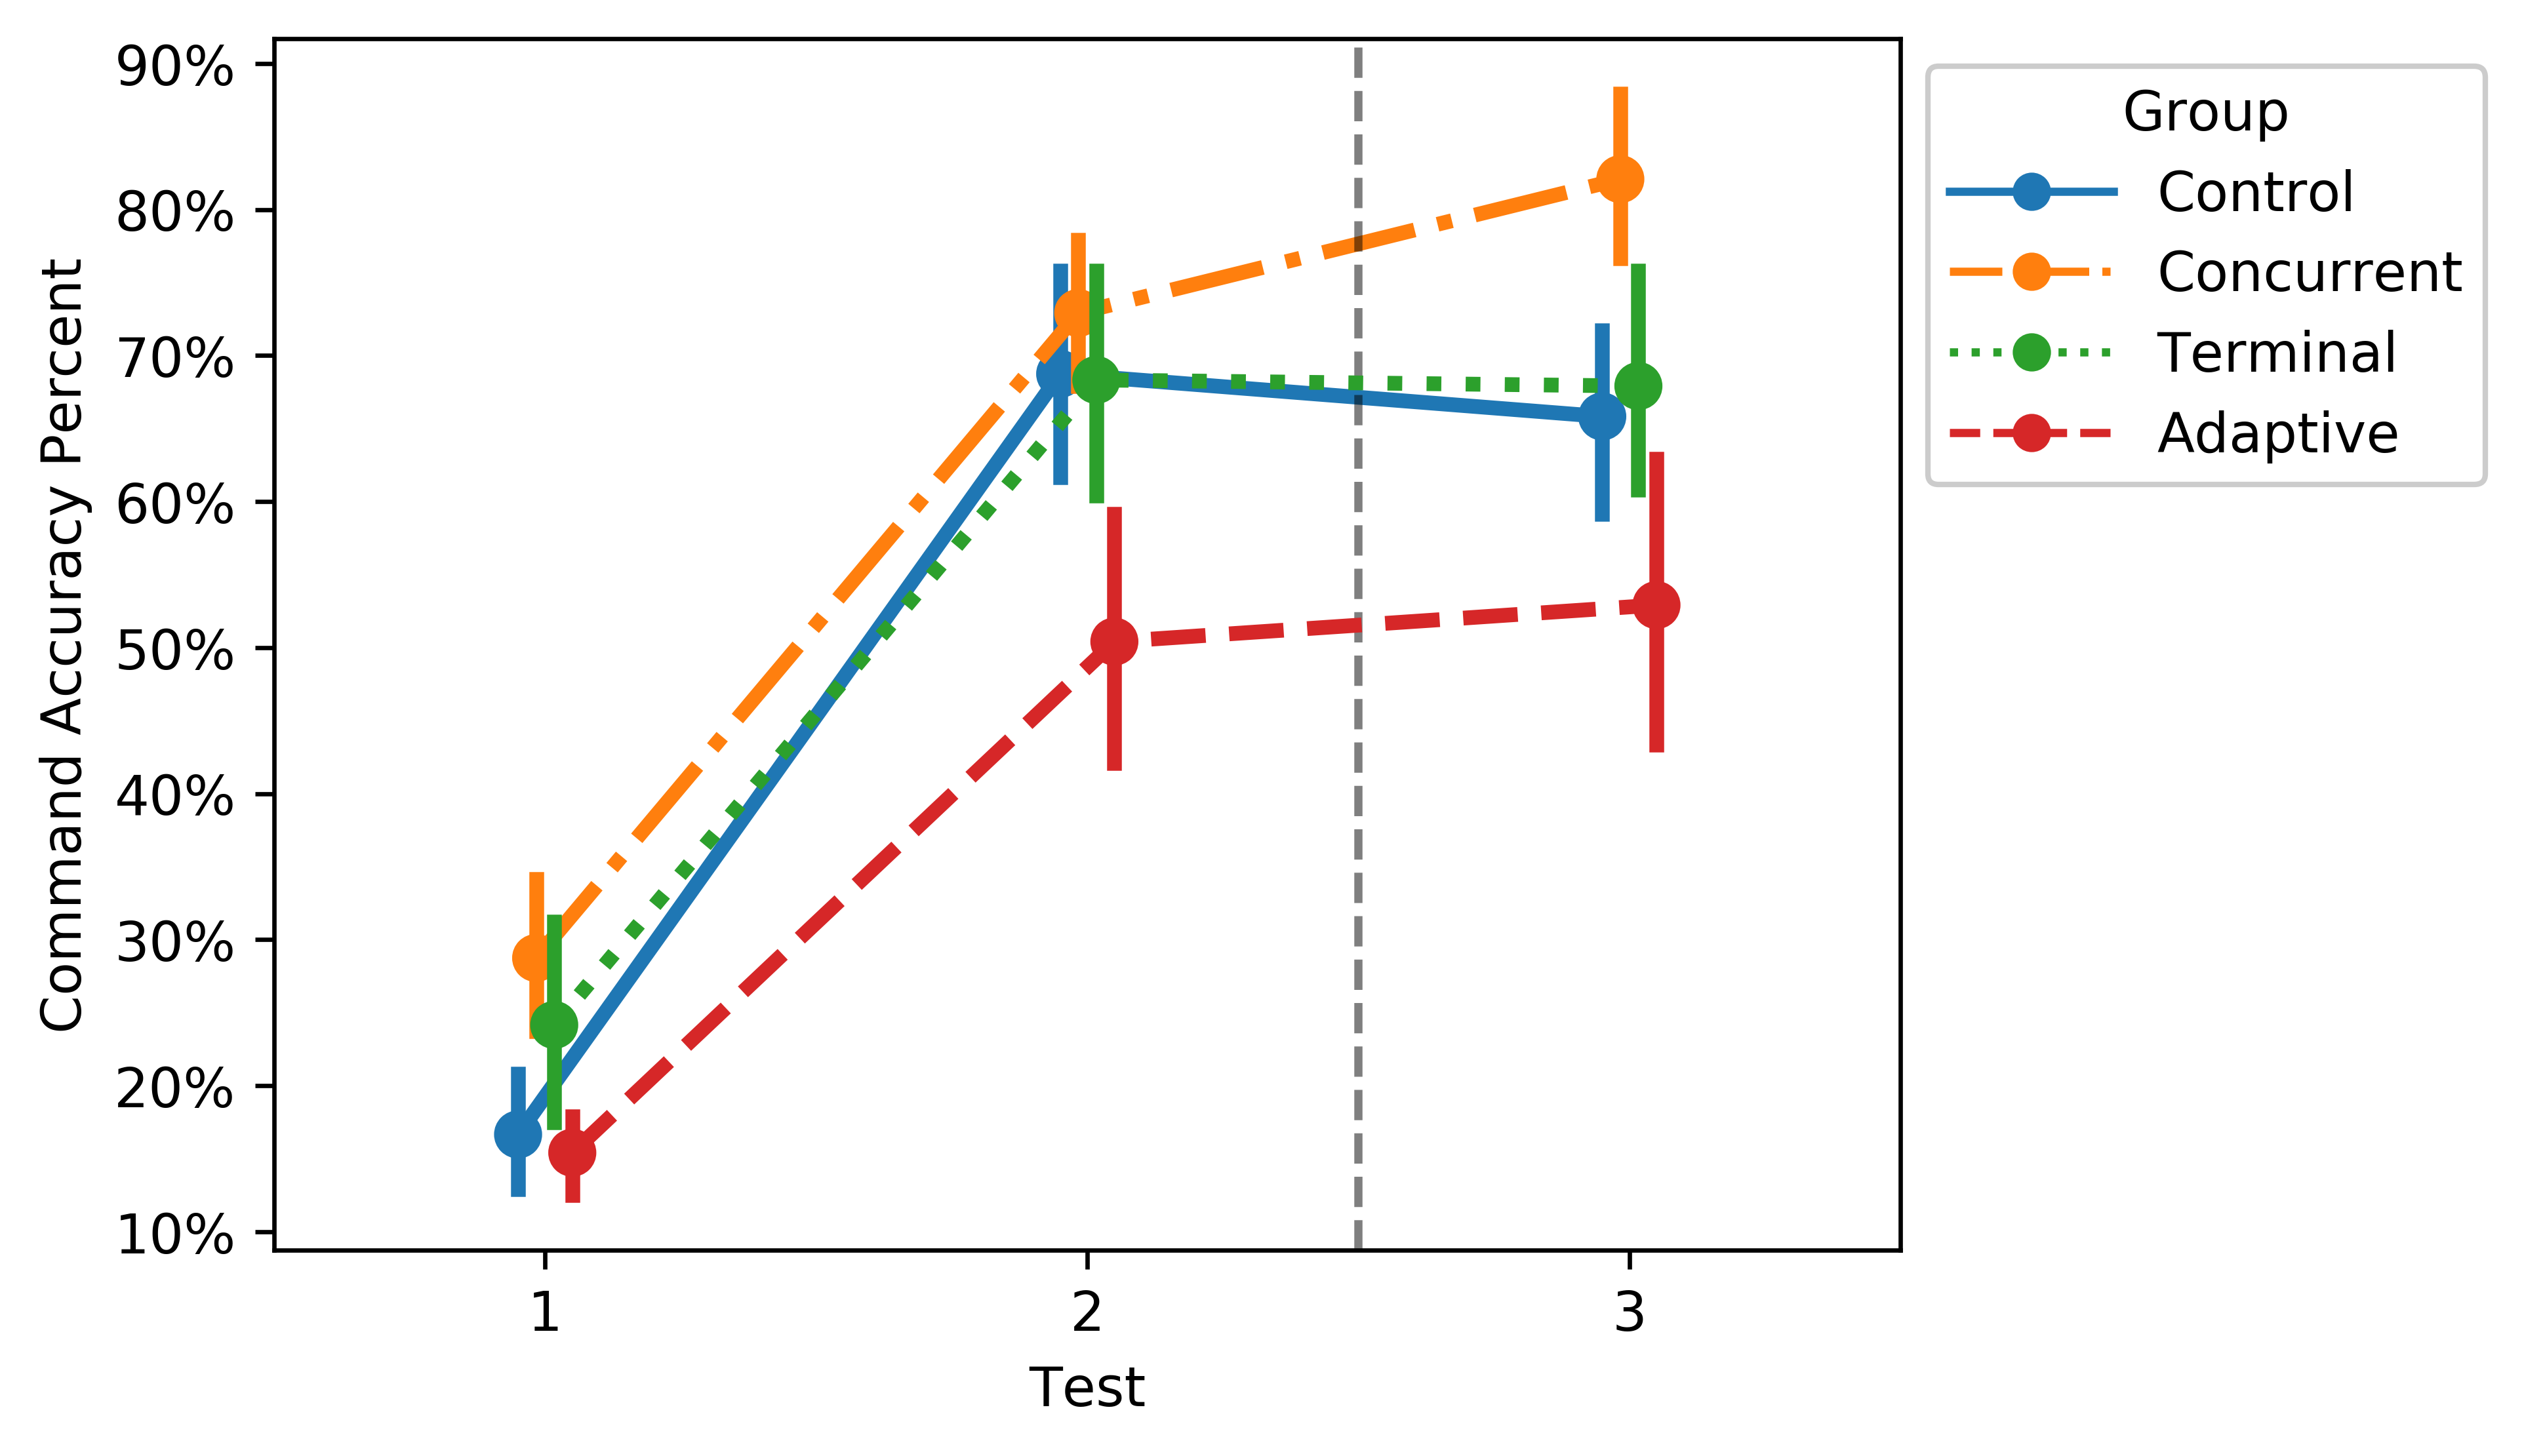
\includegraphics[height=.4\textwidth]{figures/CodeAccuracySuccess_session}
\caption{\label{figure:label7} Command Accuracy results by Test across groups.
Test 1, 2, and 3 occurred prior to the training phase, after the training phase, and after the retention phase, respectively.}
\end{figure}

\section{Discussion}
The study results elucidated a relationship between performance, workload, and trust that was influenced by the training methodology.
The Concurrent Feedback group started with the highest performance, lowest workload, and highest level of trust.
By the 5th Block, the Terminal Feedback group overlapped with the Concurrent Feedback group in terms of percent success, workload, and trust.
These two groups then tracked each other for the remainder of the study.
The Concurrent Feedback and Terminal Feedback groups did not have significantly different average trial times throughout the study.
The initial learning of these two groups differed with the Concurrent Feedback group demonstrating high performance with smaller, incremental gains and the Terminal Feedback group with larger Block-to-Block improvements.
The Control and Adaptive Threshold groups did not appear to reach a performance plateau for the percent success and steadily improved in subsequent Blocks.
Interestingly, the trust score also continually increased for both the Control and Adaptive Threshold groups.
Although the changing cursor dynamics in the Adaptive Threshold group does not seem to adversely affected trust compared to the Control group, the Adaptive Threshold group did report a significantly higher perceived workload for Blocks 9-12---the last four Blocks in the training phase.
Once the cursor dynamics stabilized, the perceived workload in the Adaptive Threshold group was not statistically different from the other groups.
These results suggested that visual feedback led to earlier performance gains with improvements in trust and workload.
The adaptive training methodology surprisingly did not adversely affect trust, but the cost was reflected in the performance and perceived workload.
Overall, all training methodologies achieved statistically similar results during the retention phase.

Measuring performance by percent success assessed the ability to complete the cursor-to-target task in the allotted 60 s.
The average trial time provided more insight into the group's performance.
The trends in the average trial time may be explained by the Command Accuracy Test results.
Higher percentages of command accuracy tracked with lower average trial times.
This relationship was expected as less time was spent attempting to input the command when the subject was able to accurately convey the inputs.
Although there were no statistically significant differences between groups in the retention phase for these metrics, it was notable that the Adaptive Threshold group consistently performed worse than the Concurrent Feedback group.

The Adaptive Threshold group did not outperform any group in any metric during the retention phase.
The results from this group were interesting for two reasons.
Firstly, an adaptive training methodology did not appear to cause adverse effects compared to the Control group.
Unreliable automation behavior can lead to poor human-automation interaction~\cite{RN54}, but was not the case in this study.
Secondly, the benefits of increased adaption induced by uncertainty did not manifest (e.g. generalization for novel tasks).
The adaption training methodology may be better tested with a different task with the same underlying structure instead of returning to a stable condition.
For example, Braun, et al.~\cite{RN36} showed that subjects trained with an adaptive training strategy were able to quickly generalize to novel tasks with similar underlying structure.
It is also possible that the cursor dynamics unpredictability was not sufficiently large compared to the inherent sEMG control noise.

Our results aligned with previously published research.
The Concurrent Feedback and Terminal Feedback groups follow the findings of Basmajian~\cite{RN27} that augmented feedback can improve performance.
We also observed effects that may be explained by Hoff and Bashir's three layer model~\cite{RN39}.
At times, there were significantly different levels of trust between the groups, which indicated that the training methodologies altered situational trust.
Subjects' trust levels also increased, which supported the notion of learned trust.
While developing a brain computer interface (BCI) was not the study objective, the throughput values during the retention phase for all groups fell within published results for sEMG cursor control systems.
Our previous single-site sEMG cursor control system with 2 DOF (counterclockwise rotation and forward) reported 2.24 bits/s and 0.23 bits/s for control methodologies that used different levels of automation~\cite{RN45}.
Multi-site systems have achieved 0.84 bits/s~\cite{RN55}, 1.3 bits/s~\cite{RN56}, and 0.4 bits/s~\cite{RN57}.
The sEMG cursor control system used in this study had a throughput of 0.56 bits/s and may be of additional interest to the BCI community.
However, the purpose of the sEMG cursor control system in this study was to provide a testbed that lent itself to motor learning adaptation and was sufficiently challenging to probe the relationship between performance, workload, and trust.

The study results largely supported our hypotheses.
The percent success performance during the training phase followed the order of Concurrent Feedback, Terminal Feedback, Control, and Adaptive Threshold, but not for all times during that phase.
All groups performed similarly in percent success during the retention phase.
The Trial completion time only supported significant differences between the Concurrent Feedback and Adaptive Threshold groups.
The subjects' trust followed our expectations with Concurrent Feedback and Terminal Feedback having the highest levels, and the Control group continually increased.
The Adaptive Threshold group had lower trust during training, and the trust increased to the level of the other groups during retention.
The workload results also supported our hypotheses that Concurrent Feedback and Terminal Feedback groups would have the largest decrease in workload, and that all groups would have similar workload during retention.
Interestingly, the Concurrent Feedback and Terminal Feedback groups converged across performance, workload, and trust by Block 5.
This study provided insights on the relationship between performance, workload, and trust for various training methodologies, and highlighted the advantage of certain methodologies during the training phase.

\section*{Acknowledgments}
The authors would like to acknowledge the subjects who took part in this study, without whom this paper would not be possible.

% \bibliography{bib}

% \end{document}
